\section{UC20 - Visualizzazione dettaglio ticket}\label{uc:20}
\paragraph{Intenzione in contesto} L'attore primario desidera visualizzare la pagina di dettaglio del ticket.

\paragraph{Attore primario} L'attore primario è o l'utente gestore o l'utente manutentore.
\paragraph{Precondizioni} L'attore primario è autenticato ed autorizzato dal sistema.
\paragraph{Post-condizioni} L'attore primario visualizza la pagina di dettaglio dei ticket di guasto.
\paragraph{Scenario principale}
\begin{enumerate}
    \item L'attore primario richiede al sistema la pagina di dettaglio del ticket di guasto;
    \item la pagina di dettaglio del ticket viene visualizzata, in particolare le informazioni relative a \hyperref[uc:20.1]{UC20.1} e \hyperref[uc:20.2]{UC20.2}.
\end{enumerate}

\begin{figure}[h]
    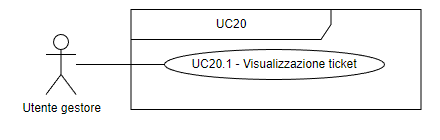
\includegraphics[width=\textwidth]{contenuti/img/casi_uso_grafici-uc20.png}
    \caption{UC20 in dettaglio}
    \label{fig:uc20}
\end{figure}


\subsection{UC20.1 - Visualizzazione titolo ticket}\label{uc:20.1}

\paragraph{Intenzione in contesto} L'attore primario vuole visualizzare il titolo del ticket;
\paragraph{Attore primario} L'attore primario è o l'utente gestore o l'utente manutentore.
\paragraph{Precondizioni}  L'attore primario è autenticato ed autorizzato dal sistema.
\paragraph{Post-condizioni} L'attore primario visualizza il titolo del ticket.
\paragraph{Scenario principale}
\begin{enumerate}
    \item L'attore primario richiede al sistema di visualizzare il titolo del ticket;
    \item il titolo del ticket è stato visualizzato.
\end{enumerate}

\subsection{UC20.2 - Visualizzazione descrizione ticket}\label{uc:20.2}

\paragraph{Intenzione in contesto} L'attore primario vuole visualizzare la descrizione testuale del ticket;
\paragraph{Attore primario} L'attore primario è o l'utente gestore o l'utente manutentore.
\paragraph{Precondizioni}  L'attore primario è autenticato ed autorizzato dal sistema.
\paragraph{Post-condizioni} L'attore primario visualizza la descrizione del ticket.
\paragraph{Scenario principale}
\begin{enumerate}
    \item L'attore primario richiede al sistema di visualizzare la descrizione del ticket;
    \item la descrizione del ticket è stata visualizzato.
\end{enumerate}